\subsection{Same-condition Component Ablations}

Table~\ref{tab:component-evidence} reports component ablations under the same species-specific splits, task inventories, training seeds, optimizer, and epoch budget as TissuePMHC. The no-branch and no-rank-fusion scores are derived from the fitted full models; the other variants are independently refitted. Task-wise comparisons use metrics averaged across seeds.

\begin{table*}[t]
\centering
\caption{Formal same-condition ablations on the Human and Mouse occurrence-matched fixed tests. AUROC and AUPRC are task-macro mean $\pm$ sample standard deviation across seeds 20260704--20260706. $\Delta$ AUROC is candidate minus the full model after averaging each task across seeds; brackets give a 10,000-resample task-bootstrap 95\% confidence interval. W/T/L counts tasks with positive/zero/negative deltas. Two-sided paired Wilcoxon $p$-values are Holm-adjusted over the four component contrasts separately within each species. Human has 77 tasks and Mouse has 11.}
\label{tab:component-evidence}
\fontsize{7.2}{8.2}\selectfont
\setlength{\tabcolsep}{1.8pt}
\begin{tabularx}{\textwidth}{@{}l>{\raggedright\arraybackslash}Xrrr>{\raggedleft\arraybackslash}p{2.35cm}rr@{}}
\toprule
Species & System & AUROC & AUPRC & $\Delta$ AUROC & 95\% CI & W/T/L & Holm $p$ \\
\midrule
Human & Full TissuePMHC & $0.8136\pm0.0021$ & $0.8126\pm0.0021$ & --- & --- & --- & --- \\
& No MHC-specific branch & $0.7923\pm0.0017$ & $0.7913\pm0.0014$ & $-0.0213$ & [$-0.0265,-0.0164$] & 11/0/66 & $4.45\times10^{-10}$ \\
& No within-task rank fusion & $0.8115\pm0.0027$ & $0.8117\pm0.0022$ & $-0.0021$ & [$-0.0036,-0.0007$] & 29/0/48 & 0.0111 \\
& No auxiliary supervision & $0.8169\pm0.0023$ & $0.8156\pm0.0025$ & $+0.0033$ & [$-0.0017,+0.0080$] & 45/0/32 & 0.1793 \\
& No multi-kernel encoder & $0.7999\pm0.0037$ & $0.7989\pm0.0036$ & $-0.0137$ & [$-0.0189,-0.0084$] & 19/0/58 & $2.13\times10^{-5}$ \\
\midrule
Mouse & Full TissuePMHC & $0.8194\pm0.0157$ & $0.8279\pm0.0121$ & --- & --- & --- & --- \\
& No MHC-specific branch & $0.8133\pm0.0142$ & $0.8218\pm0.0074$ & $-0.0061$ & [$-0.0144,+0.0017$] & 4/0/7 & 0.2783 \\
& No within-task rank fusion & $0.8163\pm0.0160$ & $0.8254\pm0.0124$ & $-0.0032$ & [$-0.0067,+0.0006$] & 3/0/8 & 0.2031 \\
& No auxiliary supervision & $0.8098\pm0.0147$ & $0.8233\pm0.0141$ & $-0.0096$ & [$-0.0155,-0.0035$] & 2/0/9 & 0.0732 \\
& No multi-kernel encoder & $0.7949\pm0.0178$ & $0.8043\pm0.0159$ & $-0.0245$ & [$-0.0333,-0.0148$] & 1/0/10 & 0.0117 \\
\bottomrule
\end{tabularx}
\end{table*}

The multi-kernel encoder contributes in both species: replacing it with a position-preserving flattened MLP lowers AUROC by 0.0137 in human and 0.0245 in mouse. Removing the MHC-specific pathway lowers human AUROC by 0.0213, supporting complementary global and allele-restricted sharing; the mouse effect is directionally similar but imprecise across 11 tasks. Rank fusion provides a smaller human gain, whereas auxiliary supervision shows no corrected benefit in either species. These are predictive component effects, not assignments of biological function to individual branches.

\subsection{Post-hoc Sequence Attribution in Human}

The Expected Integrated Gradients implementation reproduces all 23,100 saved per-seed human fixed-test scores exactly and passes branch-level completeness audits. Residue--position summaries are also stable across initializations (median pairwise Spearman \(r=0.8577\)).

Figure~\ref{fig:shap-paired-position} summarizes 1,540 complete fixed-test pairs. The largest branch-consensus differences occur at P2 (0.6425 logit attribution), P3 (0.4686), and P9 (0.3067), with the same ordering in both pathways. The P2--P3 concentration and secondary P9 peak show that the fitted model relies strongly on short N-terminal patterns and a C-terminal anchor position. These are model-used positions rather than causal biological effects.

\begin{figure}[t]
\centering

\includegraphics[width=\columnwidth]{figures/figure8_shap_paired_position.pdf}
\caption{Pair-matched positional attribution for the tuned Human model. For each of 77 tissue--HLA tasks, 20 complete test pairs are explained under three seeds. Blue circles and vermilion squares show the recorded-positive minus matched-negative observed-residue attribution for the global and HLA-specific pathways; vertical ranges connect the two pathway values, and navy diamonds show their descriptive consensus. Shaded bands emphasize P2, P3, and P9. Values are branch-logit approximations from task-conditional Expected Integrated Gradients; the consensus does not exactly decompose percentile-rank fusion.}
\label{fig:shap-paired-position}
\end{figure}

HLA-stratified maps further show that these positions do not reflect one pooled residue pattern (Supplementary Figure~\ref{S-fig:shap-hla-motifs}). For example, HLA-A*02:01 favors distinct P2 and P9 residues, whereas HLA-A*24:02 and HLA-B*07:02 show different structures, supporting an allele-associated sequence interpretation.

\subsection{Single-residue Perturbation Validation}

To test model response directly, we scored all 526,680 single-amino-acid substitutions on the explained test rows. Reloaded checkpoints reproduce the saved branch scores and percentile-rank fusion to numerical precision.

Figure~\ref{fig:ism-validation}a independently recovers the Expected-IG attribution ordering: P2 is most sensitive (0.1759 mean absolute rank-fusion change), followed by P3 (0.1066) and P9 (0.1056). Mean P2/P9 sensitivity exceeds that of the other positions by 0.0590 (95\% CI 0.0566--0.0615). This supports the pooled position-level result without implying identical anchor chemistry across HLAs.

Expected-IG attribution correlates strongly with mean ISM mutation loss (Spearman \(\rho=0.827\) for the global pathway and \(0.911\) for the HLA-specific pathway; Figure~\ref{fig:ism-validation}b--c). Exact substitution effects are less stable across seeds than the P2/P3/P9 ordering, so ISM supports the positional pattern rather than a fixed catalogue of beneficial or deleterious substitutions.

\begin{figure*}[t]
\centering
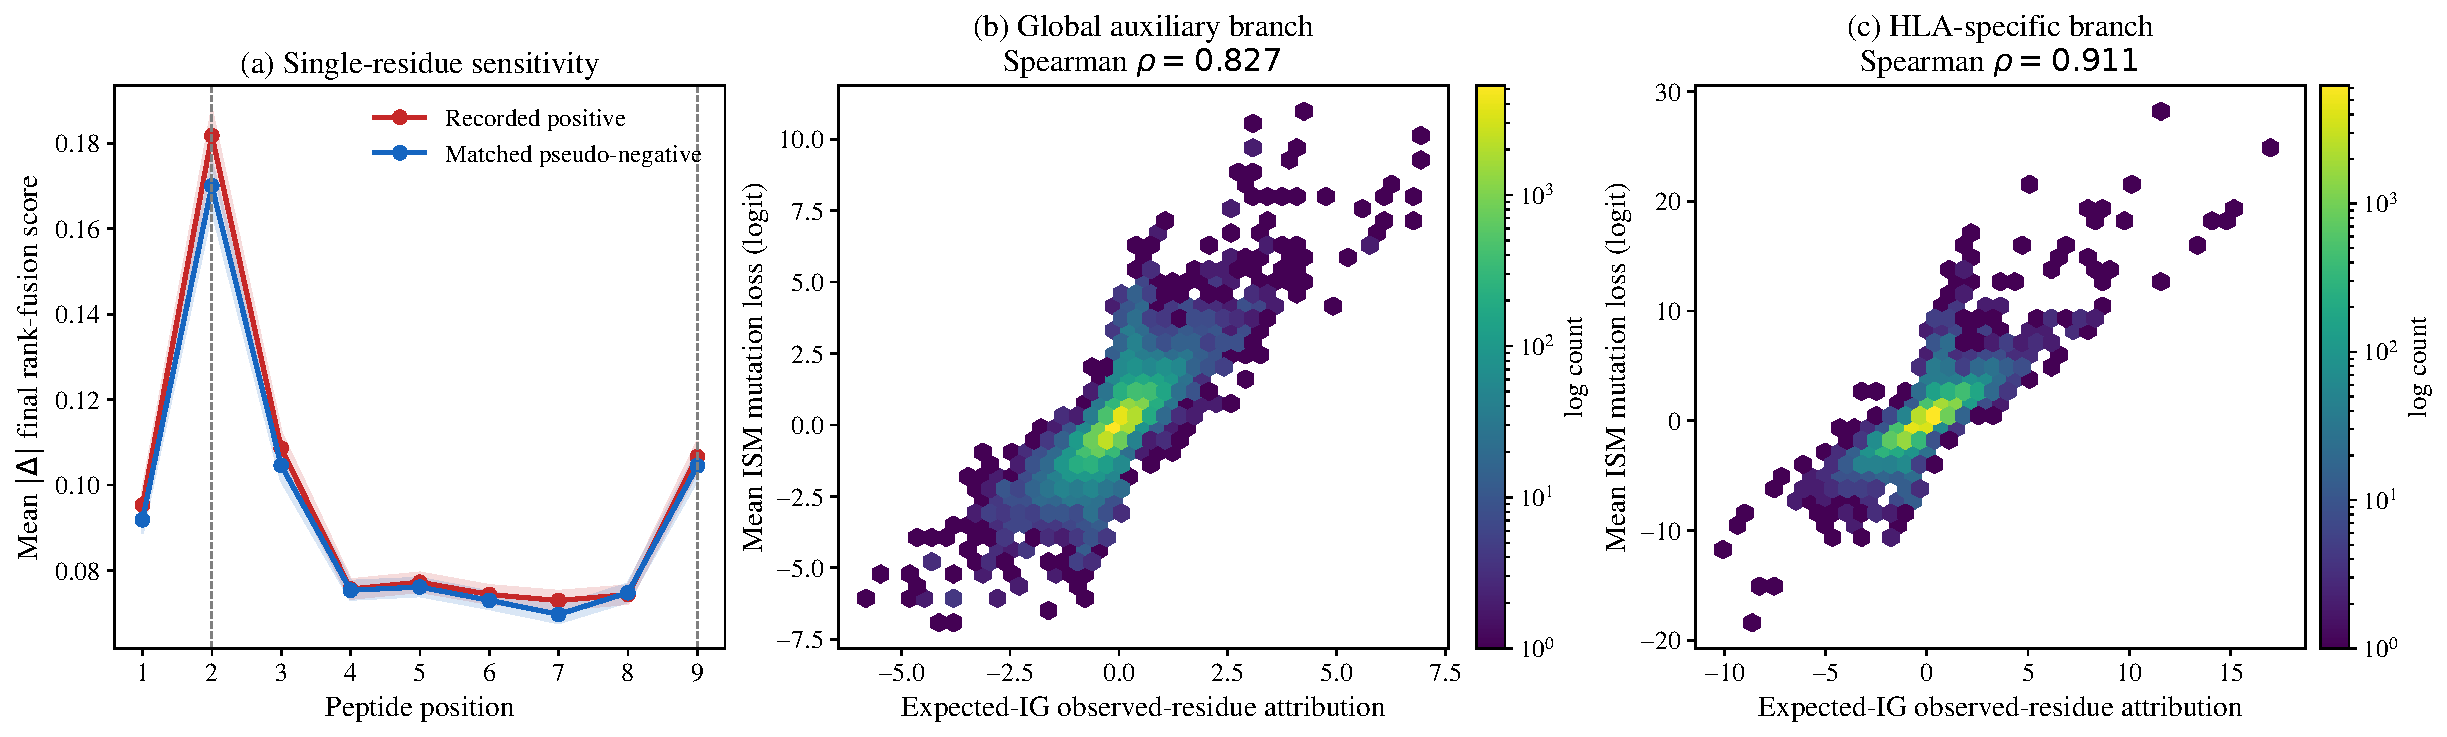
\includegraphics[width=0.95\textwidth]{figures/figure10_ism_validation.pdf}
\caption{Exhaustive single-residue in silico mutagenesis (ISM) validation. (a) Mean absolute change in the final within-task rank-fusion score over 19 substitutions, averaged across three seeds; bands show 95\% intervals over peptides. (b--c) Observed-residue Expected-IG attribution versus mean ISM branch-logit loss for the global and HLA-specific pathways. ISM measures fitted-model response to computational substitutions, not an in vivo mutation effect.}
\label{fig:ism-validation}
\end{figure*}

Switching only the tissue task also changes predicted substitution effects. Across 28 multi-tissue HLA alleles, the mean same-HLA difference between tissue tasks is 0.1703, compared with 0.0871 across seeds within a task; tissue dispersion exceeds seed dispersion for every allele. Mutation-effect rankings often change direction as well as magnitude (median same-HLA tissue-pair Spearman \(\rho=-0.266\); sign disagreement 0.596). Supplementary Figure~\ref{S-fig:cross-tissue-ism} provides the full analysis.
